\documentclass[a4paper]{article}

\usepackage[english]{babel}
\usepackage[utf8]{inputenc}
\usepackage{amsfonts}

\usepackage{amsmath}
\usepackage{graphicx}
\usepackage[colorinlistoftodos]{todonotes}

\title{dsPIC33: Exercise}
\author{Pierre Gerard, Julian Schrembi, Francois Schiltz}

\setlength{\parindent}{0pt}

\begin{document}
\maketitle

\section{Question 1}

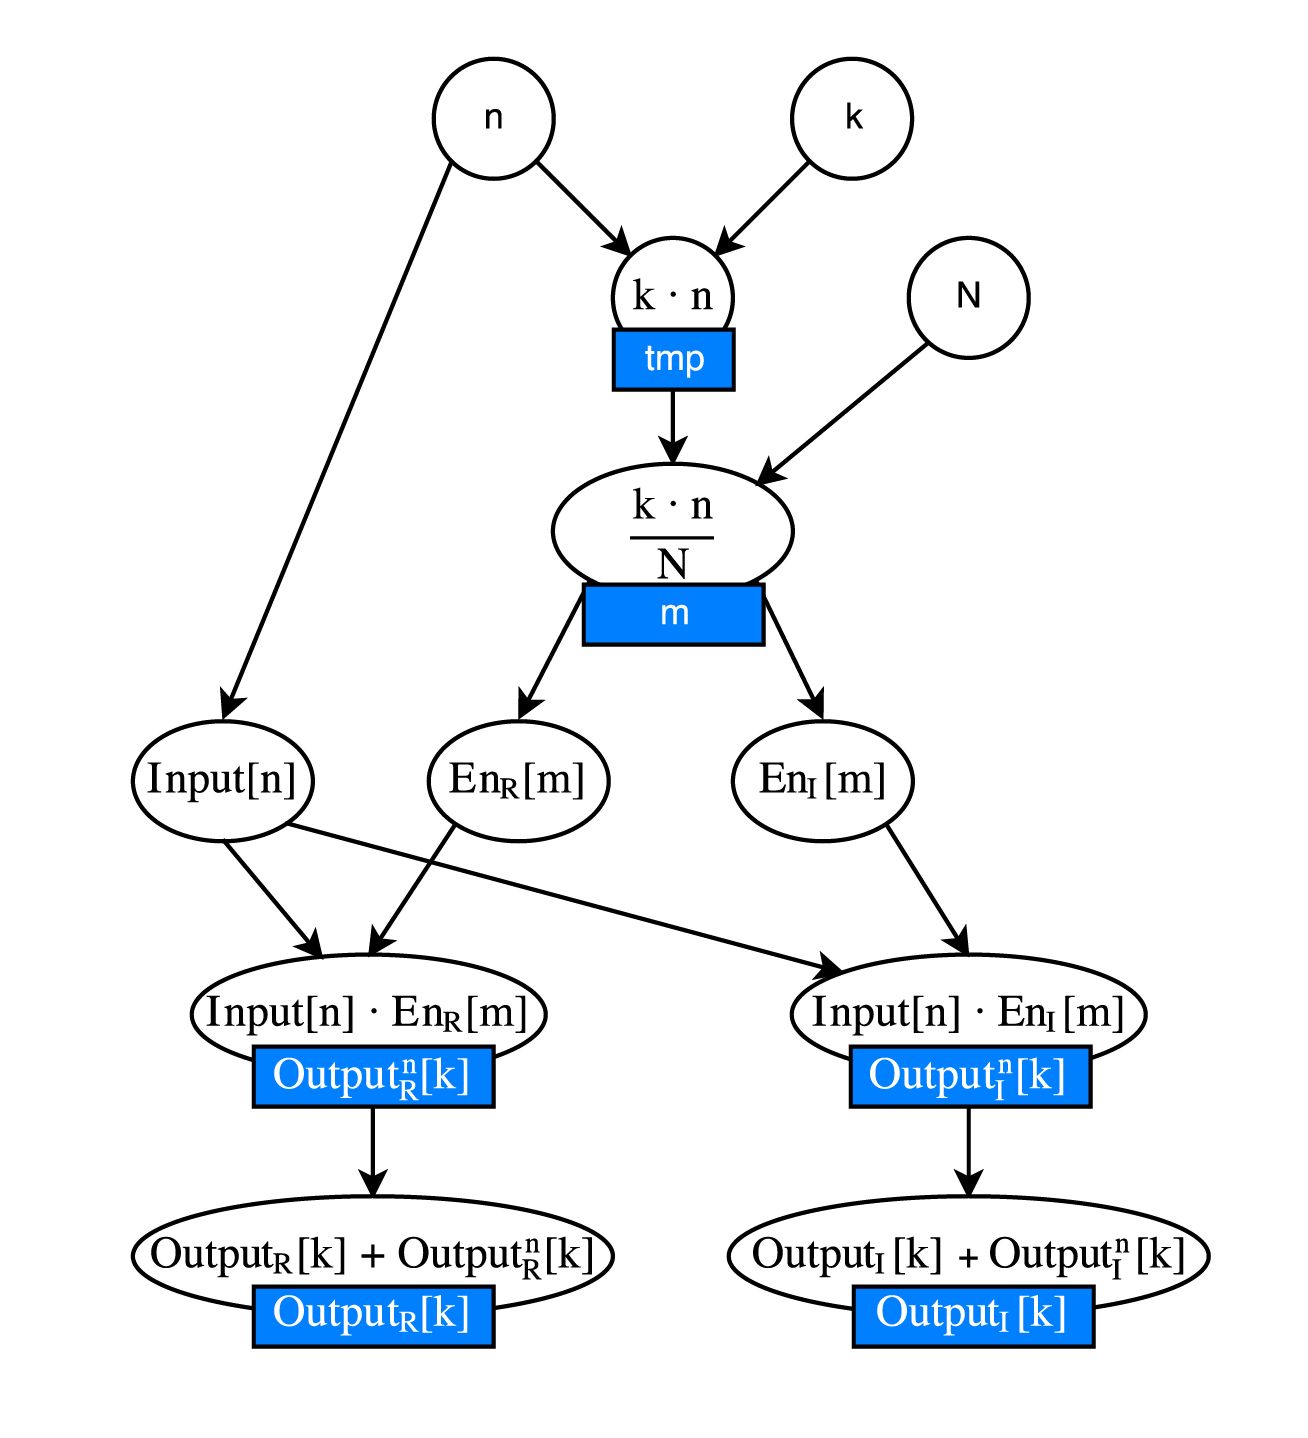
\includegraphics[scale=1]{files/elect-01.png} 

\section{Question 2}

\subsection{Computation of the value m}


\verb|INT16U unsigned16temp;|

\verb|unsigned16temp = (k * n);|

\verb|m = (INT8U) (unsigned16temp / (INT16U) N);|
\\

If we directly do the computation $ m = k*n/N $ we would get a wrong result. In fact the multiplication would be too big some the result would overflow and be wrong. To solve that problem, we use a intermediate var of 16bit to store the result of the multiplication and then do the division and then cast it back to 8 bits, the cast should be correct because the result of the division should stands on 8bits if the inputs are correct.

\subsection{Computation of the real part}

\verb|signed16temp_r = (INT16S)input[n] * (INT16S) en_r[m];|
\\
First we cast the 8 bits fixed point integer to two 16bits fixed point integer and then do the multiplication as shown in the $example2.c$. We put the result in a 16bits integer so the result would be correct\\
\verb|signed8temp = (signed16temp_r+128) >> 8;|
\\
Then we are required to put the result in a 8 bits register so to get better result we first round it  and then do the shift to get the most significant bits
\\
\verb|signed16temp_r = (INT16S) signed8temp + (INT16S) output_r[k];|
\\
% TODO a verifier si c'est bon ..

\subsection{Computation of the imaginary part}

Actually it is the same as the real part with other variable name


\section{Question 3}

\subsection{Computation of the value m}

\verb|unsigned16temp = (k * n);|

Since we do INT16 = INT8 * INT8 no overflow will occur. Let's take a look at a borderline case :   $ 1111\ 1111 * 1111\ 1111 = 1111\ 1110\ 0000\ 0001 $. There is no information lost so the accuracy is maximum.

\verb|m = (INT8U) (unsigned16temp / (INT16U) N);|

If the input are in there correct range, no overflow will occur because m must be between 0 and 127 included, so it is ok to cast it to a 8 bit integer. Some precision can be lost during the division since the result is a integer all the time. Plus it loose the decimal, so for instance $1.9$ will be $1$ if interpreted as an integer instead of 2 for the nearest integer. Let's take a look at another (non-trivial) borderline case :   $ 0000\ 0001 * 0000\ 0001\ /\ N = 0000\ 0000\ 0000\ 0001 / 128 \Leftrightarrow 0000\ 0000\ 0000\ 0001 \gg 8 = 0000\ 0000 $.

\subsection{Computation of the real part}

%TODO

\subsection{Computation of the imaginary part}

%TODO


\verb INT16S = INT8S * INT8S


\section{Question 4}
The more the frequency grows, the nearest the sample are. So that mean that two sample will have almost the same value. From a certain point, we might see that the sample will have the same value.

% TODO est ce qu'ils veulent une valeur précise ?

\end{document}